\section{Overview}\label{subsec:overview}
We start by considering the company structure introduced in Figure~\ref{company_structure}.

\begin{figure}[ht!]
\centering
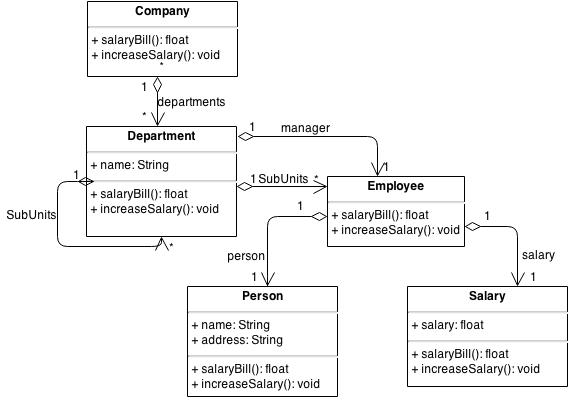
\includegraphics[width=90mm]{Company.jpg}
\caption{Company Structure \label{company_structure}}
\end{figure}

\subsection{Object Oriented Solution}

A very natural Object-Oriented way to model the company structure is as illustrated in Figure~\ref{oop_company} and Figure~\ref{oop_salary}. Similar code can be applied to Department, Employee, SubUnit and Person. A Company comprises a list of Departments. Each Department is managed by an Employee as the manager and contains a list of SubUnits. The SubUnit can be either a department or an Employee. An Employee is a Person with the Salary Information. 

\begin{figure}[tb]
\lstinputlisting[linerange=6-17]{../ObjectAlgebras/src/sybDemo1/Company.java} % APPLY:linerange=OOP_COMPANY
\vspace{-.1in}
\caption{Company Class of OOP style}
\label{oop_company}
\end{figure}

\begin{figure}[tb]
\lstinputlisting[linerange=4-9]{../ObjectAlgebras/src/sybDemo1/Salary.java} % APPLY:linerange=OOP_SALARY
\vspace{-.1in}
\caption{Salary Class of OOP style}
\label{oop_salary}
\end{figure}

Now consider adding two operations to our company structure: query the salary bill for the whole company and increase the salary of each employee by 10\%. The methods Float salaryBill() and void increaseSalary() in Figure~\ref{oop_company} and Figure~\ref{oop_salary} is an easy solution. 

This way of Object Oriented style representation of tree structures can become cumbersome and inflexible due to the bound relationship between classes. For instance, adding a new operation such as pretty printing of the company structure requires a lot of changes on the existing code and violates the no modification rule. 

\subsection{Modeling Company Structure with Object Algebras}
Object Algebras is a good solution to solve the extensibility problem. Figure~\ref{syb_tree} shows the approach to model the Company structure with Object Algebras. 
\begin{figure}[tb]
\lstinputlisting[linerange=8-17]{../ObjectAlgebras/src/trees/SybAlg.java} % APPLY:linerange=SYB_TREE
\vspace{-.1in}
\caption{Company Structure represented by Object Algebra Interface}
\label{syb_tree}
\end{figure}

Hence different operations can be realized by inheriting object algebras from the object algebra interface. To implement query bill operation for the whole Company structure, we can implement the Company interface with specific operation for each component. 
\begin{lstlisting}[numbers=none] 
public class SalaryQuerySybAlg implements SybAlg<Float,Float,Float,Float,Float,Float> {
	public Float C(List<Float> depts){
		Float r = 0f;
		for (Float f: depts) r += f;
		return r;
	}
	...
	public Float S(float salary){
		return salary;
	}
}
\end{lstlisting}

While IncreaseSalary can be realized as: 
\begin{lstlisting}[numbers=none]
public class IncreaseSalarySybAlg implements SybAlg<Float, Float, Float, Float, Float, Float> {
	public SybAlg<Float, Float, Float, Float, Float, Float> alg;
	public IncreaseSalarySybAlg(SybAlg<Float, Float, Float, Float, Float, Float> alg) { this.alg = alg; }
	public Float C(List<Float> depts) {
		return alg.C(depts);
	}
	...
	public Float S(float salary) {
		return alg.S(salary*1.1f);
	}
}
\end{lstlisting}
An increase salary algebra is used to raise the salary for each employee based on a given algebra. 

However, although we solved the problem of extensibility with object algebras, the traversal code become so long and most of the time we are writing boilerplate routine code, which is to call the methods of its child leaves. The only code we are really interested in is the Salary S(Float salary) method to return or to increase the salary. It will be great if we can design some generic classes for queries and transformations. Hence specific algebras can be generated by implementing interesting cases of generic queries and transformations. Moreover, it will be even better if the boilerplate code can be generated automatically so we can focus our attention on the interesting cases. 

\subsection{Object Algebra Framework}
Motivated by this problem of writing generic code for tree structure traversals, we introduce generic queries and transformations for Object Algebras, which can be easily inherited by real cases of queries and transformations. Furthermore, we designed an object algebra framework with great features. With our framework, the generic query and transformation classes can be generated automatically by adding an ``$@$Algebra'' annotation. 

Now with our Object Algebra Framework, the code we need to write for Salary Bill and Increase Salary will be much shorter. A Generic query code will be as short as Figure~\ref{query_with_oaframework}. 
\begin{figure}[tb]
\lstinputlisting[linerange=8-11]{../ObjectAlgebras/src/example_SybAlg/FloatQuery.java} % APPLY:linerange=QUERY_WITH_OAFRAMEWORK
\vspace{-.1in}
\caption{Query Salary Class with Object Algebra Framework}
\label{query_with_oaframework}
\end{figure}
Transformation code will be like Figure~\ref{transform_with_oaframework}
\begin{figure}[tb]
\lstinputlisting[linerange=7-12]{../ObjectAlgebras/src/example_SybAlg/IncSalary.java} % APPLY:linerange=TRANSFORM_WITH_OAFRAMEWORK
\vspace{-.1in}
\caption{Increase Salary Class with Object Algebra Framework}
\label{transform_with_oaframework}
\end{figure}
The classes SybAlgQuery<R>, SybAlgTransform<R,R,R,R,R,R> are generated by the framework automatically. 